\input{text/diss}
\usepackage{setspace}
\usepackage{colortbl}
\usepackage{lscape}
\usepackage{booktabs,array}
\newcolumntype{C}{>{\centering\arraybackslash}m{5em}}

\def\labauthors{Понур К.А., Сарафанов Ф.Г., Сидоров Д.А.}
\def\labgroup{$20.49^2$}
\def\labnumber{$14.7309^2$}
\def\labtheme{Изучение интерференции в схеме с бипризмой Френеля}
\renewcommand{\vec}{\mathbf}
\renewcommand{\Re}{\operatorname{Re}}
\renewcommand{\Im}{\operatorname{Im}}
\renewcommand{\phi}{\phi}
\renewcommand{\kappa}{\varkappa}
\renewcommand{\hat}{\widehat}
\renewcommand{\epsilon}{\varepsilon}
\renewcommand{\phi}{\varphi}
\begin{document}

%%%%%%%%%%%%%%%%%%%%%%%%%%%%%%%%%%%%%%%%%%%%%%%%%%%%%%%%%%%%%%%%%%%%%%%%%%%%%%%
\input{text/titlepage}
%%%%%%%%%%%%%%%%%%%%%%%%%%%%%%%%%%%%%%%%%%%%%%%%%%%%%%%%%%%%%%%%%%%%%%%%%%%%%%%
\begin{spacing}{1}
\tableofcontents
\end{spacing}
% \setstretch{1.2}
\newpage
%%%%%%%%%%%%%%%%%%%%%%%%%%%%%%%%%%%%%%%%%%%%%%%%%%%%%%%%%%%%%%%%%%%%%%%%%%%%%%%


 \section{Изучение интерференции в схеме с бипризмой Френеля}
\subsection{Введение}

Цель работы -- целью данной работы является получение интерфереционной картины, проверка некоторых теоретических формул
и определение средней длины волны света, пропускаемого красным и зеленым светофильтрами.
В данной работе для получения когерентных источников света применяется способ, предложенный Френелем и связанный с использованием бипризмы.
\subsection{Теоретическая часть}
В произвольной точке экрана результирующая интенсивность $I(x)$ есть усредненное за время регистрации $\tau$ значение квадрата напряженности суммарного электрического поля:
\begin{gather}
\label{eq:1}
	\vec{E}(r,t)=\vec{E_1}(r_1,t)+\vec{E_2}(r_2,t)=\\=
	-\vec{A_1}(r_1)\cos(\omega t-kr_1+\phi_1)+\vec{A_2}(r_2)
		\cos(\omega t -kr_2+\phi_2), \text{то есть} \nonumber
\end{gather}
\begin{equation}
	I(x)=A_1^2+A_2^2+2(\vec{A_1},\vec{A_2})\cos[k(r_2-r_1-(\phi_2-\phi_1)]
\end{equation}
Бипризма представляет собой две соединенные своими основаниями призмы с одинаковыми и очень малыми (порядка долей градуса) преломляющими углами. 

Каждая из половинок бипризмы отклоняет падающие на неё лучи к своему основанию и поворачивает тем самым фронт волны.  Продолжения лучей, отклоненных первой половиной бипризмы, пересекаются в точке $S_1$, которую можно рассматривать как мнимый источник света. Продолжения всех лучей, отконенных второй половиной бипризмы, пересекаются в точке $S_2$, которую можно рассматривать как другой мнимый источник света. Так как лучи, отклоненные обеими половинками бипризмы, падают на неё от одногои того же источника света, то мнимые источники света $S_1$ и $S_2$ будут когерентны. 

Та область, в которой распространяет- ся волне, отклоненная одной только первой половиной бипризмы, на рис. 3 заштрихована линиями, параллельными $OA$. Та область, в которой распространяется волна, отклоненная одной только второй половиной бипризмы, заштрихована линиями, параллельными $OB$. В области $OMN$ , покрытой на рис. 3 двойной
штриховкой, происходит наложение двух когерентных волн от двух мнимых источников $S_1$, и $S_2$. В этой области пространства имеют место явления интерференции и на участке $MN$ экрана
наблюдения мы увидим ряд светлых и темных (при освещении белым светом - окрашенных) интерференционных полос.

\begin{figure}[H]
	\centering
	\includegraphics[width=0.55\textwidth]{ris/ris3}
	\caption{ }
	\label{fig:ris3}
\end{figure}

При построении хода лучей, отклоняемых бипризмой (\ref{fig:ris3}) в случае малого преломляющего угла ы. бипризмы и малых углов падения лучей на призму можно воспользоваться следующей приближенной формулой для угла отклонения $\epsilon$
Согласно этому выражению угол отклонении призмой лучей в рассматриваемом приближении не зависит от угля падения и целиком определяется материалом и геометрией призмы. Так, например, если показатель преломления стекла, из которого сделана бипризма, $n=1.5$, то угол отклонения $\epsilon$ просто равен половине преломляющего угла $\alpha$ призмы:
\begin{equation}
 	\epsilon=\frac{\alpha}{2}
 \end{equation} 

Воспользовавшись формулой $s$ или $s$ и выполнив построение хода лучей, можно убедиться в том, что, если $SO\bot AB$ (\ref{fig:ris3}), то мнимые изображения и	действительного источника света $S$ лежат в одной плоскости с действительным источником, причем эта плоскость параллельна передней грани бипризмы. Это обстоятельство в дальнейшем облегчит нам нахождение расстояния $\delta$ между мнимыми источниками $S_1$ и	$S_2$.
Ограничения поля интерференции $MN$ за бипризмой зависят от величины предельного угла расходимости $\phi_0$ светового пучка, падающего на бипризму от щели $S$. Особый интерес представляют два частных случая:

1. При $\phi_0 = 2\epsilon$	линейная ширина поля интерференции,
начиная с расстояния $h$ за бипризмой, остается неизменной и равна расстоянию $\delta$ между мнимыми источниками $S_1$ и $S_2$.

2. При $h\rightarrow\infty$,что можно осуществить,
осветив бипризму параллельным пучком лучей, полученным с помощью вспомогательной линзы (\ref{fig:ris4}), сечение поля интерференции имеет форму ромба. Максимальная ширина поля интерференции $MN$ в этом случае равна половине ширины параллельного пучка падающего на бипризму. Такая схема интерференции соответствует cлучаю наложения двух параллельных когерентных световых пучков
пересекающих друг друга под постоянным углом.
\begin{figure}[H]
	\centering
	\includegraphics[width=0.85\textwidth]{ris/ris4}
	\caption{ }
	\label{fig:ris2}
\end{figure}
Для расчета наблюдаемой на экране интерференционной картины воспользуемся тем, что бипризма Френеля так изменяет ход лучей от действительного источника, что дает нам право рассматривать световое возмущение в области $MN$ (\ref{fig:ris3}) как результат синфазного излучения двух мнимых источников $S_1$ и $S_2$. При этом рассматривая выражение (\ref{eq:1})для соответствующих проекций $\vec{E_1}(r,t)$ $\vec{E_2}(r,t)$, пренебрежем зависимостью амплитуд $A_1$ и $A_2$ от расстояния $r$, то есть будем считать $A_1=A_2=A_0$	и положим $\phi_1=\phi_2=0$.

Найдем как ширина $d$ полос интерференции зависит от параметров нашей измерительной установки, то есть от длины установки $L$,расстояния между мнимыми источниками и длины волны света  
$\lambda$, испускаемого действиткльным источником $S$. В точку $P$ на экране $MN$ колебания источников $S_1$ и $S_2$ придут с разностью хода:
\begin{equation}
	\Delta=S_2B=r_2-r_1
\end{equation}
и, следовательно, с разностью фаз
\begin{equation}
	\phi(x)=\frac{2\pi}{\lambda}(r_2-r_1)
\end{equation}
На основании вышеизложенного и в соответствии с выражением (\ref{eq:1}) интенсивность результирующего колебания в точке наблюдения $P$ с координатой $x$ определяется формулой
\begin{equation}
	I(x)=2A^2[1+\cos{\phi(x)}]=A^2\cos^2{\frac{\phi}{2}}
\end{equation}
Максимумы освещенности будут получаться в тех местах экрана, для которых разность фаз
\begin{equation}
	\phi(x)=\frac{2\pi}{\lambda}\Delta=2\pi m, \text{где} m=0;\pm 1,\pm 2,\cdots
\end{equation}
То есть для которых разность хода
\begin{equation}
	\Delta=r_2-r_1=m\lambda
\end{equation}

Для нахождения координат максимумов интенсивности вычислим разность хода $\Delta=r_2-r_1$. Несложно получить: 
\begin{gather}
	\label{eq:8}
	r_2-r_1=\frac{4ax}{r_1+r_2} \\ \nonumber
	r_1^2=L^2+(x-a)^2 \\ \nonumber
	r_2^2=L^2+(x+a)^2 \nonumber
\end{gather}


Предполагая величины $\frac{x+a}{L}$ и $\frac{x-a}{L}$ малыми, разложим $r_1$ и $r_2$ в ряд и ограничимся двумя членами в разложении. В результате получим
\begin{equation}
	\label{eq:9}
	r_1+r_2\simeq 2L +\frac{x^2+a^2}{L} 
\end{equation}
Подставляя (\ref{eq:9}) в (\ref{eq:8}) найдём, что 
\begin{equation}
	r_2-r_1\simeq \frac{2ax}{L}\left(1-\frac{x^1+a^2}{2l^2} \right) \label{eq:10}
\end{equation}
При условии 
\begin{equation}
	\frac{\delta x(x^2+a^2)}{2L^3}\ll\frac{\lambda}{2}
\end{equation}
которое позволяет в выражении для разности хода (\ref{eq:10}) отбросить слагаемое, дающее малый по сравнению с $\pi$ вклад в разность фаз интерфеиррующих волн, точное выражение (\ref{eq:8}) может быть заменено на приближенное
\begin{equation}
 	r_1-r_2\simeq\frac{\delta x}{L} \label{eq:12}
 \end{equation} 
 Отметим, что выражение (\ref{eq:12}) сразу следует при условии малости угла 
 $\theta (\sin{\theta}\simeq\theta)$ из приближения приближения парралельных лучей. 
 \begin{equation}
 	\Delta=S_2C=\delta\sin{\theta}\simeq\frac{\delta x}{L}
 \end{equation}
 Следовательно, ширина полос интерференции, равная расстоянию между двумя соседними максимумами освещенности в первои приближении равна:
 \begin{equation}
 	x_{m+1}-x_m=d=\frac{L\lambda}{\delta} \label{eq:14}
 \end{equation}
 Формулу (\ref{eq:14}), переписанную в другом виде
 \begin{equation}
 	\delta d=L\lambda
 \end{equation}
 удобно использовать для проверки теории интерференционных явлений. Если оставлять неизменным расстояние $L$ между щелью $S$ и экраном наблюдения и работать с одной и той же длиной волны $\lambda$ (пользоваться одним и тем же светофильтром), то произведение $\delta d$ должно оставаться (согласно теории) постоянным. Таким образом, для проверки теории нужно, меняя расстояние между мнимыми источниками, независимыми способами измерять расстояния $\delta$ и $d$.Если их произведение будет оставаться постоянным (конечно, при $L= \const$ и $\lambda=\const$ ), то это будет служить доказательством правильности изложенной теории. Расстояние $\delta$ между мнимыми источниками в данной работе можно изменять, изменяя величину $h$ (см. рис. ). То есть помещая бипризму на различным расстояниях от щели.
%%%%%%%%%%%%%%%%%%%%%%%%%%%%%%%%%%%%%%%%%%%%%%%%%%%%%%%%%%%%%%%%%%%%%%%%%%%%%%%
\section{Практическая часть}
\subsection{Задание 1}
Качественно пронаблюдали зависимость между $d$ и $h$: с возрастанием $h$ $d$ уменьшается.

Были измерены предельные значения ширины щели $\Delta x$ и ширины интерфереционной полосы $d$ при минимальном и максимальном значении $h$, при которых происходило размытие картины: 
\begin{gather*}
h_{min}\to d=0.80\text{ мм}, \quad \Delta x=-0.06\text{ мм}\\
h_{max}\to d=0.13\text{ мм}, \quad \Delta x=1.95\text{ мм} 	
\end{gather*}

Из геомерии можно получить зависимость сдвига интерфереционной картины $\xi$ от положения источника над главной оптической осью $\varkappa$: 
\begin{equation}
	\xi=\varkappa \frac{L-h}{L}
\end{equation}
Будем считать интерференционную картину размытой, когда максимумы, приходящие от противоположных концов щели, будут сдвинуты на половину пространственного периода:	
\begin{equation}
	2\xi=\frac{d}{4}
\end{equation}
Отсюда выражаем максимальную ширину щели:
\begin{equation}
	\text{Ш}=2\varkappa=\frac{hd}{2(L-h)}
\end{equation}

Например, для $h_{min}=0.80\text{ мм}$ мы имеет ширину щели $\Delta x=0.09 \text{мм}$

\newpage
\subsection{Задание 2}
Из подобия треугольников можно получить формулу для вычисления расстояния между мниными источниками 
\begin{equation}
	\delta=\frac{l_1}{l_2}\cdot b
\end{equation}
Были произведены измерения $\delta$ и $d$ при нескольких $h$ при постоянном $L$ с красным светофильтром:
\input{tables/red2}
\begin{figure}[H]
	\centering 
	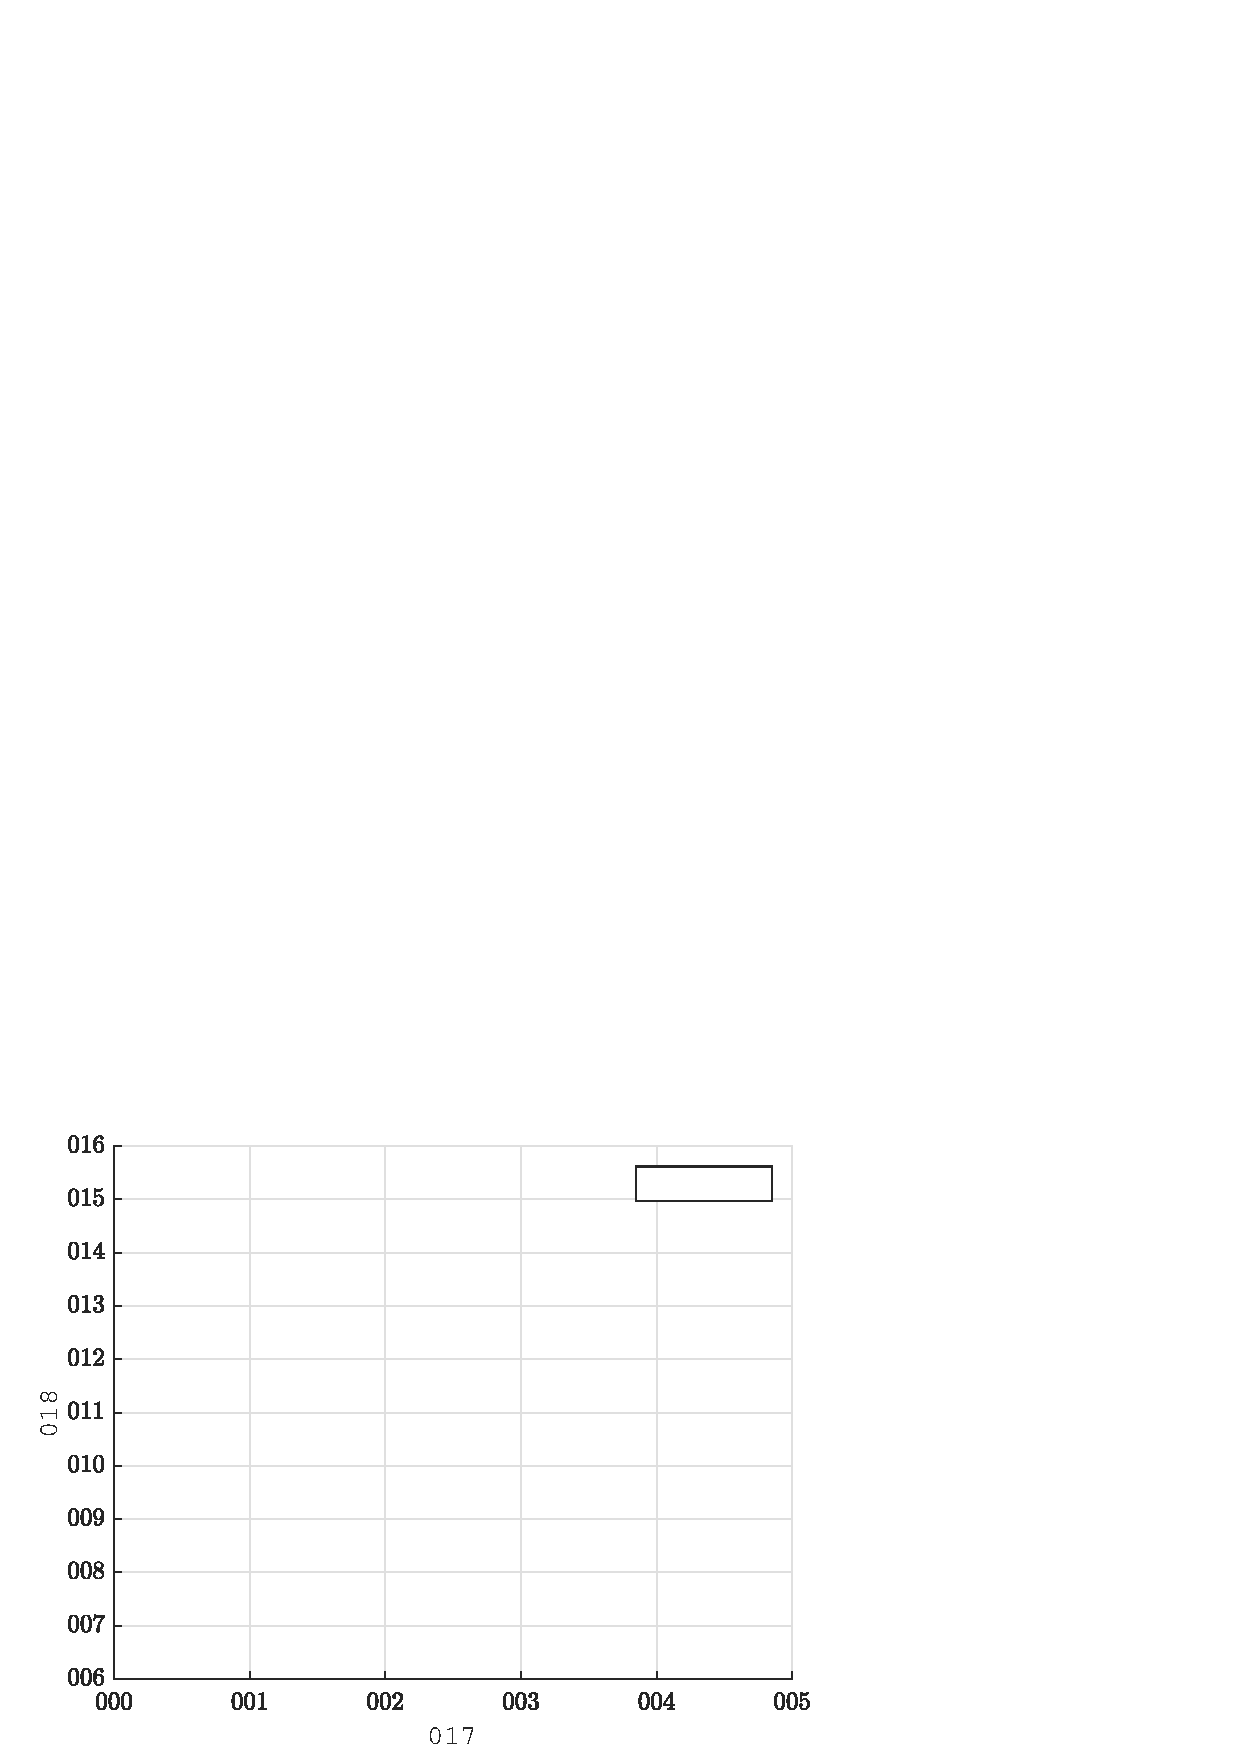
\includegraphics[width=0.995\textwidth]{data/d_r.png}
	\caption{Красный светофильтр}
	\label{fig:d_r}
\end{figure}

И с зеленым светофильтром:
\input{tables/green2}
\begin{figure}[H]
	\centering
	\includegraphics[width=1\textwidth]{data/d_g.png}
	\caption{Зеленый светофильтр}
	\label{fig:d_g}
\end{figure}

По экспериментальным данным построили графики зависимости $\delta\cdot d$ и $\delta$ от $h$:
\begin{figure}[H]
	\centering
	\includegraphics[width=0.8\textwidth]{data/dd_r.png}
	\caption{Красный светофильтр}
	\label{fig:dd_r}
\end{figure}

\begin{figure}[H]
	\centering
	\includegraphics[width=0.8\textwidth]{data/dd_g.png}
	\caption{Зеленый светофильтр}
	\label{fig:dd_g}
\end{figure}

Из графика определили среднюю длину волны:
\begin{gather*}
	\mean{\lambda_\text{зел}}=531 \text{ нм}\\
	\mean{\lambda_\text{кр}}=634 \text{ нм}
\end{gather*}
% По полученным данным построили графиги:


 % \begin{figure}[]
% 	\centering
% 	\includegraphics[width=0.\textwidth]{data/dd_r.png}
% 	\caption{}
% 	\label{fig:dd_r}
% \end{figure}
% \begin{figure}[]
% 	\centering
% 	\includegraphics[width=0.\textwidth]{data/dd_g.png}
% 	\caption{}
% 	\label{fig:dr_g}
% \end{figure}
\subsection{Задание 3}
Также из подобия треугольников выводится формула зависимости количества полос $N$ от расстояния $h$ от источника до призмы:
\begin{gather}
	N=\frac{2\delta(L-h)}{dh} \nonumber
\end{gather}
При этом необходимо учесть, что $\delta(h)=2\epsilon h$. Тогда получаем 
\begin{equation}
	N=2\frac{\epsilon^2(Lh-h^2)}{L\lambda}
\end{equation}
Функция принимает максимальное значение при $h=L/2$.

Примерно определили порядок следования цветов при интерфереции в белом свете:
\begin{equation}
	\text{Красный--Желтый--Зеленый--Синий}
\end{equation}

Это, очевидно, следует из того, что  с изменением длины волны изменяется пространственный период интерфереционной картины, а так как максимумы линейно зависят от длины волны, то мы можем наблюдать их чередование в интерфереционной картине.  

Мы сняли зависимость $N(h)$ и сопоставили с теоретической, где наблюдали хорошее совпадение теории с практикой:
\input{tables/tab3-1}
\begin{figure}[H]
	\centering
	\includegraphics[width=0.8\textwidth]{data/N_r.png}
	\caption{Красный светофильтр}
	\label{fig:dd_g}
\end{figure}
\begin{figure}[H]
	\centering
	\includegraphics[width=0.8\textwidth]{data/N_g.png}
	\caption{Зеленый светофильтр}
	\label{fig:N_g}
\end{figure}

\subsection{Задание 4}
На оптической скамье была собрана установка по схеме, изображенной на рисунке (рис. \ref{fig:ris2}). Сняли зависимость ширины поля интерференции $MN$ и числа интерференционных полос от расстояния между бипризмой	 и экраном $y$:

\input{tables/tab4-2}

Так как с помощью дополнительной линзы пучок был сделан более-менее параллельным, то изменение ширины полос $d$ с изменением $y$ было незначительным и уложилось в пределы погрешности.

Используя формулу 
\begin{equation}
	d=\frac{\lambda}{2\epsilon}	
\end{equation}
можно вычислить угол $\epsilon$ под которым в данном случае сходятся интерфереционные лучи. Используя средние значения длин волн, которые были найдены выше, получаем
\begin{gather*}
	\epsilon_{\text{кр}}\simeq\epsilon_{\text{зел}}=0.00132
\end{gather*}
 Найденное ранне значение $\epsilon=0.00121$

\section{Заключение}
Мы ознакомились с установкой,отъюстировали её, качественно пронаблюдали зависимость между $d$ и $h$: с возрастанием $h$ уменьшается $d$. Были измерены предельные значения ширины щели и ширины интерфереционной полосы при минимальном и максимальном значении $h$: 
\begin{gather*}
h_{min}\to d=0.80\text{ мм}, \quad \Delta x=-0.06\text{ мм}\\
h_{max}\to d=0.13\text{ мм}, \quad \Delta x=1.95\text{ мм} 	
\end{gather*}
   
\end{document} 